\documentclass[11pt, a4paper, reqno]{scrartcl}

\usepackage[utf8]{inputenc}
\usepackage{a4wide}
\usepackage{libertine}
\usepackage{graphicx}
\usepackage{listings}
\usepackage{xcolor}
\usepackage{float}
\usepackage{amsmath}
\usepackage{microtype}

% for latex output of pandas
\usepackage{booktabs}

\begin{document}
    \title{Computational Statistics and Data Analysis\\Sheet No. 4}
    \author{David Bubeck, Patrick Nisbl\`e}
    \maketitle

    \lstset{
        language=R,
        backgroundcolor=\color{gray!5},
        numbers=left,
        captionpos=t,
        breaklines=true,
        frame=l,
        xleftmargin=\parindent,
        basicstyle=\footnotesize\sffamily,
        keywordstyle=\bfseries\color{green!40!black},
        commentstyle=\itshape\color{purple!40!black},
        identifierstyle=\color{blue!60!black},
        stringstyle=\color{orange}
    }

    \section{Unit Circle}
        We are to create uniformly distributed points in a unit circle and show the values for $z_1$ and $z_2$ are gaussian distributed
        
        \begin{figure}[H]
            \lstinputlisting{ex1.R}
            \caption{ex1.R}
        \end{figure}
    
        \begin{figure}[H]
            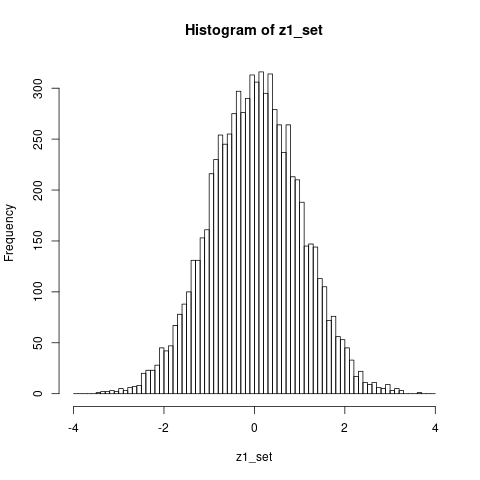
\includegraphics[width=.7\paperwidth]{ex1.png}
        \end{figure}
        
        
\end{document}
